\documentclass[english,master]{liumaiex}
% Options are english, swedish, bachelor and master


%=========================================================================%
%
% Add optional packages. Some are almost essential. 
%
%=========================================================================%
\usepackage{amssymb}
\usepackage{amsmath}
\usepackage[dvips]{graphicx}
\usepackage{xcolor}
\usepackage{amsthm}
\usepackage{comment}
\usepackage{parskip}
\usepackage{tikz}
\usepackage{lipsum}

\theoremstyle{plain}
\newtheorem{proposition}{Proposition}[section]
\newtheorem{corollary}[proposition]{Corollary}
\newtheorem{lemma}[proposition]{Lemma}
\newtheorem{theorem}[proposition]{Theorem}
\newtheorem{conjecture}[proposition]{Conjecture}
\theoremstyle{definition}
\newtheorem{definition}[proposition]{Definition}
\newtheorem{example}[proposition]{Example}
\newtheorem{remark}[proposition]{Remark}

\newcommand\todo[1]{\textcolor{red}{#1}}
\newcommand{\sgn}{\text{sgn}}
\newcommand{\tr}{\text{tr}}

\begin{document}


%=========================================================================%
%
% Information to fill-in
%
%=========================================================================%
\title{The title of the thesis}
\author{Erik Jonasson}
\shortauthor{Jonasson}
% If there are several authors, just enter the names separated by comma or 'and'
\publishmonth{June}
\publishyear{2024}
%\city{City} % Has Linköping as default
%\department{Department name} % Has MAI as default
\supervisor*{Hans Lundmark}
% To add another supervisor, just use the command again
\examiner*{Fredrik Andersson} % use a star to add department automatically
% \supervisor also accepts the star format
%\level{G2} % Not needed when bachelor/master is set in options
%\credits{16 hp} % Not needed when bachelor/master is set in options
\regnumber{The number your thesis gets from administrators}
\enkeywords{Keyword 1, keyword 2, etc.}
\svkeywords{Nyckelord 1, nyckelord 2, etc.}
\publishurl{The url to the thesis}
%\pdfauthor{Name} % Needed if name is complex
%\pdftitle{Title} % Needed if title is complex
%\pdfkeywords{Keywords} % Needed if keywords are complex
%\pdfsubject{Subject} % Optional

\maketitle


%=========================================================================%
%
% Introductory part: Abstract, Acknowledgements, etc 
%
%=========================================================================%
\pagenumbering{roman}
\section*{Abstract}

A summary of the thesis, presenting the important results.

\placeenkeywords
\placeenurl

\newpage

% \cleardoublepage
% \begin{otherlanguage*}{swedish}
% \chapter*{Sammanfattning}

% You can write a swedish abstract in this environment to get
% correct (swedish) formatting and hyphenation

% \placesvkeywords
% \placesvurl
% \end{otherlanguage*}

% \chapter*{Acknowledgements}

% Acknowledgements and thanks to people that have helped you.

% \chapter*{Nomenclature}

% The notation you will use in the thesis

\tableofcontents
%\listoffigures
%\listoftables

\newpage



%=========================================================================%
%
% Main part of the thesis
%
%=========================================================================%
\pagenumbering{arabic}

\section{Introduction}

\subsection{Background}

The starting point of this thesis is the Novikov equation
\begin{equation} \label{eq:Novikov}
	m_t + ((um)_x + 2u_xm) u = 0,\quad m = u - u_{xx}.
\end{equation}
The Novikov equation belongs to a family of equations known as peakon equations. These are integrable systems, which are non-linear differential equations where the solutions can be reduced to a finite number of algebraic operations and integrations. Such systems are rare, as most non-linear differential equations lack explicit solutions. Solitons are a type of wave that can propagate and interact with other solitons without changing shape. Solitons were first discovered in nature by John Scott Russell in 1834 when he observed a solitary wave in a canal. They have since been studied in many fields such as fluid dynamics, optics, and quantum mechanics.

In 1895, Korteweg and de Vries discovered the a soliton equation, the Korteweg--de Vries (KdV) equation \sloppy
\begin{equation}
	u_t + u_{xxx} - 6uu_x = 0.	
\end{equation}
The KdV equation is a partial differential equation that describes the waves in shallow water. It was not until much later that Zabusky and Kruskal \cite{Zabusky1965} discovered in numerically in 1965 that the KdV equation has soliton solutions. In 1993, Camassa and Holm discovered the Camassa--Holm \cite{Camassa_1993} equation
\begin{equation} \label{eq:CH}
	m_t + (um)_x + u_xm = 0,\quad m = u - u_{xx},
\end{equation}
which was the first equation with peaked soliton solutions. These solutions have are one the following form
\begin{equation} \label{eq:peakon}
	u(x, t) = \sum_{k = 1}^{N} m_k(t) e^{-|x - x_k(t)|}.
\end{equation}
The peakon solutions differs from the KdV equations soliton solutions in that they have a sharp peak. Later the Degasperis--Procesi equation
\begin{equation} \label{eq:DP}
	m_t + (um)_x + 2u_xm = 0,\quad m = u - u_{xx}.
\end{equation}
was discovered by Degasperis and Procesi in 1999 \cite{Degasperis_1999}. Both the CH and DP equations share similar properties with the Novikov equation. For a more detailed discussion of the peakon equations and its properties, see the comprehensive overview by Lundmark and Szmigielski \cite{Lundmark_2022}.

This brings us back to the Novikov equation. It was discovered by Vladimir Novikov in a classification of cubically nonlinear PDEs admitting infinitely many symmetries \cite{Novikov_2009}, with Hone and Wang \cite{Hone2008} later providing a Lax pair for it.

The focus of the thesis is on the high-frequency limit of the Novikov equation. The high-frequency limit is obtained by substitution of $x \mapsto \epsilon x$, $t \mapsto \epsilon t$, and letting $\epsilon \rightarrow 0$. This limit gives the following equation
\begin{equation} \label{eq:Novikov_high_freq}
	m_t + ((um)_x + 2u_xm) u = 0,\quad m = u_{xx}.
\end{equation}
which is the same as the Novikov equation, but with $m = u_{xx}$ instead of $m = u - u_{xx}$. Both the CH and DP equations have been studied in the high-frequency limit, and it has been shown that they yield piecewise linear solutions. The high-frequency limit of the Novikov equation is expected to yield similar piecewise linear solutions. The high frequency limit of the Camassa--Holm equation yields the Hunter--Saxton equation \cite{HunterSaxton_1991,HunterZheng1994} for nematic liquid crystals. The high frequency limit of the Degasperis--Procesi equation yields the derivative Burgers equation \cite{Kohlenberg_2007, Lundmark_2008}.
\begin{center}
  \begin{tabular}{c|c}
    $m=u-u_{xx}$ & $m=u_{xx}$ \\
    \hline
    Camassa--Holm & Hunter--Saxton \\
    \hline
    Degasperis--Procesi & Derivative Burgers \\
    \hline
    Novikov & HF Novikov \\
  \end{tabular}
\end{center}

The high-frequency limit of the CH and DP equations have piecewise linear solutions on the following form
\begin{equation} \label{eq:linear_peakon}
	u(x, t) = \sum_{k = 1}^{N} m_k(t) |x - x_k(t)|.
\end{equation}
So we will make the assumption that the high frequency limit of the Novikov equation will have a similar piecewise linear solution.

The time derivative of $x_k$ and $m_k$ will be governed by the following ODEs
\begin{equation} \label{eq:peakon_odes}
\dot{x}_k = u(x_k)^2, \quad
\dot{m}_k = -m_ku_x(x_k)u(x_k).
\end{equation}
Dots denote $\frac{d}{dt}$ as usual. $u(x_k)$ and $u(x = x_k,t)$ is given by
\begin{align}
	u(x_k) &= \sum_{i = 1}^{N} m_i(t) |x_k - x_i(t)|, \\
	u_x(x_k) &= \sum_{i = 1}^{N} m_i(t) \sgn(x_k - x_i).
\end{align}
See Appendix(\ref{sec:DerivationODE}) for the proof of that ODE-system is compatible with the PDE. The time derivatives of $x_k$ and $m_k$ for the original Novikov equation have the same form, but then $u$ is the peakon equation (\ref{eq:peakon}) instead of the linear equation (\ref{eq:linear_peakon}).

\section{Preliminaries}

\subsection{Lax pairs}

Lax pairs are a mathematical framework used to analyze and solve certain types of integrable systems. They are the main tool used to solve peakon equations. The concept of Lax pairs was introduced by Peter Lax in 1968 \cite{Lax_1968}. A Lax Pair consists of two operators, $L$ and $A$, that satisfy a specific compatibility condition. The existence of a Lax Pair for a nonlinear PDE is a strong indicator of the equation's integrability. It allows the application of powerful analytical methods to find exact solutions and conservation laws. In many cases, Lax pairs are represented in matrix form, enabling a more straightforward application of the IST method.

\subsubsection*{Zero curvature representation}

The zero curvature representation is a generalization of the Lax pair, consisting of a pair of linear equations
\begin{equation}
	\partial_x \psi = U \psi, \quad \partial_t \psi = V \psi,
\end{equation}
that satisfy the zero curvature condition
\begin{equation}
	\partial_t U - \partial_x V + [U, V] = 0.
\end{equation}
The condition comes from equating the mixed partials $\partial_t \partial_x \psi = \partial_x \partial_t \psi$. The matrices $U$ and $V$ are called the Lax pair. The zero curvature condition is only satisfied if the Lax pair is integrable. 
\begin{example}
The KdV has the following Lax pair
\begin{subequations}
  \begin{equation}
    \frac{\partial}{\partial x} \psi =
    \begin{pmatrix}
      0 & 1 \\
      u - \lambda & 0
    \end{pmatrix}
	\psi,
  \end{equation}
  \begin{equation}
    \frac{\partial}{\partial t} \psi =
    \begin{pmatrix}
      -u_x & 2u + 4\lambda \\
      2u^2 - u_{xx} + 2u\lambda - 4\lambda^2 & u_x
    \end{pmatrix}
    \psi.
  \end{equation}
\end{subequations}
If we take the mixed partials of the Lax pair we get
\begin{equation}
	\begin{pmatrix}
	0 & 0\\
	u_t + u_{xxx} - 6u u_x & 0
	\end{pmatrix} =
	\mathbf{\bar{0}}.
\end{equation}
Which is only satisfied if the KdV equation is satisfied.
\end{example}


\subsection{Monodromy Matrix}
The Lax Pair can be used to construct the monodromy matrix \cite{Avendano2008,Krishnaswami_2021}, which is a matrix that encodes the dynamics of the system. We first need to construct the transition matrix $T$. It is defined as the solution to the linear system
\begin{equation}
	\partial_x T(y,x,t) = U(y,t) T(y,x,t), \quad T(x,x,t) = I,
\end{equation}
where U is the spatial part of the Lax pair. It describes the evolution of the system along the $x$-axis, $\psi(y,t) = T(y,x,t) \psi(x, t)$. The monodromy matrix is then defined as
\begin{equation}
	M(t) =
		\lim_{x \rightarrow \pm \infty} \lim_{y \rightarrow \pm \infty} T(y,x,t),
\end{equation}
which exist under the assumption that
\begin{equation}
	\int_{-\infty}^{\infty} ||U(y,t)|| dy < \infty.
\end{equation}
where $||\cdot||$ is some matricial norm. It can be viewed as the transition matrix of the system along the $x$-axis. The monodromy matrix is very useful for finding conserved quantities of the system.
\begin{theorem}
	\begin{equation} \label{eq:Transition-Matrix}
		\partial_t T(y,x,t) = V(y,t) T(y,x,t) - T(y,x,t) V(x,t).
	\end{equation}
\end{theorem}
\begin{proof}
	Expanding the time derivative of $T(y,x,t)$ and plugging in the zero curvature condition we get
	\begin{equation}
	\begin{aligned}
		\partial_x \partial_t T
			&= \partial_t (U) T + U \partial_t T \\
			&= \partial_t (V)T + VUT - UVT + U \partial_t T \\
			&= \partial_x (VT) + U(\partial_t T - VT) \\
	\end{aligned}
	\end{equation}
	Which is the same as
	\begin{equation}
		\partial_x (\partial_t T - VT) = U(\partial_t T - VT).
	\end{equation}
	This means that $\partial_t T - VT$ is a solution to equation \eqref{eq:Transition-Matrix}.
	This implies the existence of a non-singular matrix C, independent of x, such that
	\begin{equation}
		\partial_t T - VT = TC,
	\end{equation}
	putting $x = y$ we get
	\begin{equation}
		C(y,t) = -V(y,t),
	\end{equation}
	since $T(x,x,t) = I$.
\end{proof}
This leads to the following useful corollary
\begin{corollary} \label{cor:Monodromy}
	If $lim_{x \rightarrow \pm \infty} V(x,t) = V_0$, then
	\begin{equation}
		\partial_t M = [V_0, M].
	\end{equation}
\end{corollary}
And since the trace of a commutator is zero, the time derivative of the trace is zero.

\subsection{Hamiltonian formalism}
\todo{Todo: Add references}

The Hamiltonian formalism is a fundamental framework in classical mechanics that offers a powerful method for analyzing dynamical systems. It describes the evolution of a system with $n$ degrees of freedom in a $2n$-dimensional phase space. The state of the system is described by a set of canonical coordinates
\begin{equation}
	 (q_i,p_i), \qquad i = 1,\dots,n.
\end{equation}
In the context of the Novikov equation, the canonical coordinates are the peakon positions $x_i$ and the peakon momenta $m_i$. The Hamiltonian $H(q,p,t)$ is a functional representing the total energy or another conserved quantity of the system. It is expressed in terms of the canonical coordinates and possibly time. The evolution of the system is governed by Hamilton's equations, which take the form
%
\begin{equation}
	\dot{q}_i = \frac{\partial H}{\partial p_i}, \quad
	\dot{p}_i = -\frac{\partial H}{\partial q_i}.
\end{equation}
%
These equations describe how the abstract canonical coordinates evolve over time. A soliton PDE is integrable if it possesses as many conserved quantities $F_i$ as degrees of freedom, and these quantities are in involution
%
\begin{equation}
	\{F_i, F_j\} = 0.
\end{equation}
%
These conserved quantities allow the system's equations of motion to be solved explicitly. The canonical Hamiltonian structure can be written as
%
\begin{equation}
\begin{pmatrix}
	\dot{q} \\
	\dot{p}
\end{pmatrix} =
\begin{pmatrix}
	0 & I \\
	-I & 0
\end{pmatrix}
\begin{pmatrix}
	\partial H / \partial q \\
	\partial H / \partial p
\end{pmatrix},
\end{equation}
%
where I is the $n \times n$ identity matrix. A more general form of the Hamiltonian structure is with the $2n \times 2n$ Poisson matrix $\Pi$, where the equations of motion are instead written as
%
\begin{equation}
\begin{pmatrix}
	\dot{q} \\
	\dot{p}
\end{pmatrix} =
\Pi(x)
\begin{pmatrix}
	\partial H / \partial q \\
	\partial H / \partial p
\end{pmatrix}.
\end{equation}
%
Or as
%
\begin{equation}
	\dot{x} = \Pi(x) \nabla H(x),
\end{equation}
%
where $x = (q,p)$ and $\nabla H(x) = (\partial H / \partial q, \partial H / \partial p)$. The Poisson matrix have to be skew-symmetric, $\Pi^T = -\Pi$, and satisfy the Jacobi identity
\begin{equation}
	\{\{f,g\},h\} + \{\{g,h\},f\} + \{\{h,f\},g\} = 0.
\end{equation}
%
were the Poisson bracket for the canonical coordinates is defined as
%
\begin{align}
	\{x_i, x_j\} &= \Pi^{ij}(x), \\
	\{\{x_i, x_j\}, x_k\} &= \sum_{l=1}^n \Pi^{lk}(x) \frac{\partial}{\partial x_l} \Pi^{ij}(x).
\end{align}

\section{N = 2 solution to the high frequency limit Novikov}
The assumption that $x_1 < \cdots < x_N$ can be made without loss of generality. We can also assume that $m_k \neq 0$ since if it were equal to zero it wouldn't affect the equation. For $N = 1$, the solution is trivial since $u(x_k) = 0$, which appears in both $\dot{x}_k$ and $\dot{m}_k$. So the solution for $N=1$ is constant. For the more interesting case when $N = 2$ we get the following system of ODEs from equation \eqref{eq:peakon_odes}:
%
\begin{align}
	\dot{x}_1 & = m_2^2 (x_2 - x_1)^2, \\
	\dot{x}_2 & = m_1^2 (x_2 - x_1)^2, \\
	\dot{m}_1 & = m_1 m_2^2(x_2 - x_1),  \\
	\dot{m}_2 & = -m_1^2 m_2(x_2 - x_1).
\end{align}
%
To solve this system, we first identify conserved quantities:
\begin{align}
	(m_1^2 + m_2^2)_t = 0, \\
	(m_1m_2(x_2 - x_1))_t = 0.
\end{align}
%
To show why these are conserved, we take the time derivative of the first equation:
\begin{equation}
\begin{aligned}
	(m_1^2 + m_2^2)_t 
	&= 2m_1\dot{m}_1 + 2m_2\dot{m}_2 \\
	&= 2m_1^2m_2^2(x_2 - x_1) - 2m_1^2m_2^2(x_2 - x_1) = 0,
\end{aligned}
\end{equation}
\begin{equation}
\begin{aligned}
	(m_1m_2(x_2 - x_1))_t 
	&= \dot{m}_1m_2(x_2 - x_1) + m_1\dot{m}_2(x_2 - x_1) \\
	&- m_1m_2\dot{x}_1 + m_1m_2\dot{x}_2 \\
	&= m_1m_2^3(x_2 - x_1)^2 - m_1^3m_2(x_2 - x_1)^2 \\
	&- m_1m_2^3(x_2 - x_1)^2 + m_1^3m_2(x_2 - x_1)^2 \\
	&= 0. \\
\end{aligned}
\end{equation}
%
Denoting these conserved quantities as $M_1$ and $M_2$ respectively, we can express the conservation laws as:
\begin{align}
	m_1^2 + m_2^2 = M_1, \\
	m_1m_2(x_2 - x_1) = M_2.
\end{align}
%
Leveraging these conserved quantities, we derive expressions for $\dot{m}_1$ and $\dot{m}_2$:
\begin{equation}
\left\{ \begin{aligned}
	\dot{m}_1 = \phantom{-}m_2M_2, \\
	\dot{m}_2 = -m_1M_2.
\end{aligned} \right.
\end{equation}
%
The solutions to these equations take the form:
\begin{equation}
\left\{ \begin{aligned}
	m_1 &= \sqrt{M_1} \sin(M_2t + \phi), \\
	m_2 &= \sqrt{M_1} \cos(M_2t + \phi).
\end{aligned} \right.
\end{equation}
%
Now we can solve for $\dot{x}_1$ and $\dot{x}_2$:
\begin{align}
\left\{ \begin{aligned}
	\dot{x}_1m_1^2 = m_1^2m_2^2(x_2 - x_1) = M_2^2, \\
	\dot{x}_2m_2^2 = m_1^2m_2^2(x_2 - x_1) = M_2^2,
\end{aligned} \right. \\
\implies \left\{ \begin{aligned}
	\dot{x}_1 = \frac{M_2^2}{m_1^2} = \frac{M_2^2}{M_1\sin^2(M_2t + \phi)}, \\
	\dot{x}_2 = \frac{M_2^2}{m_2^2} = \frac{M_2^2}{M_1\cos^2(M_2t + \phi)}.
\end{aligned} \right.
\end{align}
%
Integration yields the positions:
\begin{equation}
\left\{ \begin{aligned}
	x_1 = -\frac{M_2}{M_1}\cot(M_2t + \phi) + C,\\
	x_2 = \phantom{-}\frac{M_2}{M_1}\tan(M_2t + \phi) - D.
\end{aligned} \right.
\end{equation}
%
The $M_2$ quantity implies that $D = -C$:
\begin{align}
	M_2 = m_1m_2(x_2 - x_1) = M_2 + M_1\cos(M_2t-\phi)\sin(M_2t-\phi)(C + D)).
\end{align}
%
In conclusion the piecewise solution looks like this:
\begin{align}
	u(x, t) &= m_1|x - x_1| + m_2|x - x_2|, \\
	m_1 &= \phantom{-}\sqrt{M_1} \sin(M_2t + \phi), \\
	m_2 &= \phantom{-}\sqrt{M_1} \cos(M_2t + \phi), \\
	x_1 &= -\frac{M_2}{M_1}\cot(M_2t + \phi) + C, \\
	x_2 &= \phantom{-}\frac{M_2}{M_1}\tan(M_2t + \phi) + C.
\end{align}
%
There are four constants $M_1$, $M_2$, $\phi$ and $C$, which is to be expected since we had four initial quantities, $m_1(0)$, $m_2(0)$, $x_1(0)$ and $x_2(0)$. The solution is valid only for a finite time, since we made the assumption that $x_1 < x_2$. The assumption that $x_1 < x_2$ is only valid for finite intervals since $\tan$ and $\cot$ go to infinity in a finite time.

\begin{center}
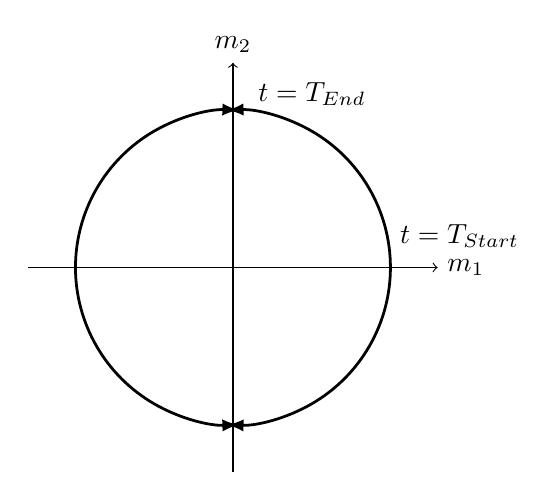
\begin{tikzpicture}[scale=2]
    % Draw the coordinate axes
    \draw[->] (-1.3,0) -- (1.3,0) node[right] {$m_1$};
    \draw[->] (0,-1.3) -- (0,1.3) node[above] {$m_2$};
    
    % Draw the circle
    % \draw (0,0) circle (1cm);

    \node[right] at (1, 0.2) {$t=T_{Start}$};
    \node[right] at (0.1, 1.1) {$t=T_{End}$};


    % Add arrows along the circle pointing to the top
    \draw[->, >=latex, line width=1pt] (0:1) arc[start angle=0,end angle=92,radius=1cm];
    \draw[->, >=latex, line width=1pt] (0:-1) arc[start angle=180,end angle=88,radius=1cm];
    \draw[->, >=latex, line width=1pt] (0:1) arc[start angle=0,end angle=-92,radius=1cm];
    \draw[->, >=latex, line width=1pt] (0:-1) arc[start angle=-180,end angle=-88,radius=1cm];
\end{tikzpicture}
\end{center}

\section{Hamiltonian structure}
\todo{Todo: Add references}

\todo{Todo: Write more}

One Hamiltonian structure of the CH equation is given by the Hamiltonian
\begin{equation}
	H(x_1, \dots, x_N, m_1, \dots, m_N) = \frac{1}{2} \sum_{i,j = 1}^{N} m_i m_j e^{-|x_i - x_j|},
\end{equation}
with a canonical Poisson bracket. The Hamiltonian structure of the Hunter Saxton equation can be derived by taking the high-frequency limit of the CH Hamiltonian structure
\begin{equation}
	H(x_1, \dots, x_N, m_1, \dots, m_N) = \frac{1}{2} \sum_{i,j = 1}^{N} m_i m_j |x_i - x_j|,
\end{equation}
with the canonical Poisson bracket.

The Hamiltonian structure of the Novikov equation is given by the same Hamiltonian as the CH equation, but with a different Poisson bracket. The Poisson bracket of the Novikov equation is given by
\begin{alignat}{3}
	\{&x_i, &x_j\} &= \sgn(x_i - x_j)(1 - e^{-2|x_i - x_j|}), \\
	\{&x_i, &m_j\} &= m_j e^{-2|x_i - x_j|}, \\
	\{&m_i, &m_j\} &= m_i m_j \sgn(x_i - x_j)e^{-2|x_i - x_j|}
\end{alignat}

A Hamiltonian structure for the high-frequency limit of the Novikov equation have not been found. One idea is to take the high-frequency limit of the Hamiltonian structure of the Novikov equation, but this does not yield the correct equations for $x_k$ and $m_k$. The Hamiltonian structure of the high-frequency limit of the Novikov equation is still an open question.

\section{Numerical analysis}
\todo{Todo: Do numerical analysis}

\section{Constants of motion}

\todo{Todo: Explain the algorithm further/better}\\
The main achievement of this thesis is the discovery of constants of motion for the high-frequency limit of the Novikov equation. Most constants have been found using an exhaustive search algorithm. The algorithm is based on the assumption that the constants of motion are polynomials in the variables $m_k$ and $x_k$ of a fixed degree $M$ and $X$ for $m_k$ respectively $x_k$. The algorithm lists all monomials of that fixed degree
\begin{equation}
	\prod_{i=1}^{N} m_i^{a_i} x_i^{b_i},
\end{equation}
where the sum of $a_i$ is $M$ and $b_i$ is $X$. The algorithm then takes the time derivative of each monomial and forms a linear combination of them. The constants of motion are then found by finding linear combinations that are zero. The algorithm have been run both symbolically in Mathematica and numerically in C++. The algorithm has been successful up until $N = 4$, where time and numerical precision becomes a limiting factor.

\subsection{Jacobian determinant method}
\todo{TODO: Give a brief overview of the Jacobian determinant method.}

\subsection*{N = 2}

\begin{align}
	M_1 &= m_1 m_2 (x_2 - x_1), \\
	M_2 &= m_1^2\phantom{x_1} + m_2^2\phantom{x_2}, \\
	M_3 &= m_1^2 x_1 + m_2^2 x_2, \\
	M_4 &= m_1^2 x_1^2 + m_2^2 x_2^2. \\
\end{align}
%
The system of ODEs for $N = 2$ only has four variables so the system should have at most three functionally independent constants of motion. We can see that
\begin{equation}
	M_1^2 = M_2M_4 - M_3^2.
\end{equation}

\subsection*{N = 3}

The algorithm have found the following five conserved quantities for $N = 3$.  The first two are
\begin{align}
	M_1 &= m_1m_2(x_2 - x_1) + m_1m_3(x_3 - x_1) + m_2m_3(x_3 - x_2), \\
	M_2 &= m_1^2m_2^2m_3^2(x_2 - x_1)(x_3 - x_1)(x_3 - x_1).
\end{align}
If we let
\begin{align}
	A & = m_1^2(M_1 + 2m_2m_3(x_3-x_2)), \\
	B & = m_2^2(M_1 + 2m_1m_3(x_3-x_1)), \\
	C & = m_3^2(M_1 + 2m_1m_2(x_2-x_1))
\end{align}
then we can write the three other conserved quantities as
\begin{align}
	M_3 &= A\phantom{x_1} + B\phantom{x_2} + C\phantom{x_3} \\
	M_4 &= Ax_1 + Bx_2 + Cx_3 \\
	M_5 &= Ax_1^2 + Bx_2^2 + Cx_3^2
\end{align}
These conserved quantities aren't functionally independent. Using the Jacobian determinant method we find that there are only four functionally independent conserved quantities. The first constant can be written as
\begin{equation}
	M_1^4 = M_3M_5 - M_4^2 + 2M_1M_2
\end{equation}

\subsection*{N = 4}

For $N = 4$ we have found six conserved quantities. The first two follow the same pattern as for $N = 3$
\begin{align}
	M_1 = &m_1 m_2 (x_2 - x_1) + m_1 m_3 (x_3 - x_1) + m_1 m_4 (x_4 - x_1) \\ +  &m_2 m_3 (x_3 - x_2) + m_2 m_4 (x_4 - x_2) + m_3 m_4 (x_4 - x_3),\\
	M_2 = &m_1^2m_2^2m_3^2m_4^2(x_2 - x_1)(x_3 - x_2)(x_4 - x_3)(x_4 - x_1).
\end{align}
For the next three let's define define the expression $W_i$ to be the sum of all the terms in $M_1$ that don't contain $m_i$. Now we can define $A, B, C, D$ as
\begin{align}
	A &= m_1^2(M_1 + 2W_1), \\
	B &= m_2^2(M_1 + 2W_2), \\
	C &= m_3^2(M_1 + 2W_3), \\
	D &= m_4^2(M_1 + 2W_4).
\end{align}
We can then write the next three conserved quantities as
\begin{align}
	M_3 =& A\phantom{x_1} + B\phantom{x_2} + C\phantom{x_3} + D\phantom{x_4} \notag \\
	&+ 6m_1m_2m_3m_4 (x_1 - x_2 + x_3 - x_4) \\
	M_4 =& Ax_1 + Bx_2 + Cx_3 + Dx_4 \notag \\
	&+ 6m_1m_2m_3m_4 (x_1x_3 - x_2x_4) \\
	M_5 =& Ax_1^2 + Bx_2^2 + Cx_3^2 + Dx_4^2 \notag \\
	&+ 6m_1m_2m_3m_4 (x_1x_2x_3 - x_1x_2x_4 + x_1x_3x_4 - x_2x_3x_4)
\end{align}
%
Interestingly, it follows very close to the pattern of the $N = 3$ case. The only difference is that we get some extra terms that all contain $m_1m_2m_3m_4$. The last found conserved quantity is
\begin{equation}
\begin{aligned}
	M_6 =
		 &m_1^2m_2^2m_3^2(x_2 - x_1)(x_3 - x_1)(x_3 - x_2) \\
		+&m_1^2m_2^2m_4^2(x_2 - x_1)(x_4 - x_1)(x_4 - x_2) \\
		+&m_1^2m_3^2m_4^2(x_3 - x_1)(x_4 - x_1)(x_4 - x_3) \\
		+&m_2^2m_3^2m_4^2(x_3 - x_2)(x_4 - x_2)(x_4 - x_2) \\
		+&2m_1^2m_2^2m_3m_4(x_4 - x_1)(x_2 - x_1)(x_3 - x_2) \\
		+&2m_1m_2^2m_3^2m_4(x_2 - x_1)(x_3 - x_2)(x_4 - x_3) \\
		+&2m_1m_2m_3^2m_4^2(x_3 - x_2)(x_4 - x_3)(x_4 - x_1) \\
		+&2m_1^2m_2m_3m_4^2(x_4 - x_3)(x_4 - x_1)(x_2 - x_1).
\end{aligned}
\end{equation}
Here we also find that all the conserved quantities aren't functionally independent. Using the Jacobian determinant method we find that there are only five functionally independent conserved quantities, but we haven't been able to find a relation between them.

\section{Zero curvature representation}

The zero curvature representation for the Novikov equation \cite{Lundmark_2022} is
\begin{subequations}
  \label{eq:Novikov-lax}
  \begin{equation}
    \label{eq:Novikov-lax-x}
    \frac{\partial}{\partial x}
    \begin{pmatrix} \psi_1 \\ \psi_2 \\ \psi_3 \end{pmatrix} =
    \begin{pmatrix}
      0 & zm & 1 \\
      0 & 0 & zm \\
      1 & 0 & 0
    \end{pmatrix}
    \begin{pmatrix} \psi_1 \\ \psi_2 \\ \psi_3 \end{pmatrix}
    ,
  \end{equation}
  \begin{equation}
    \label{eq:Novikov-lax-t}
    \frac{\partial}{\partial t}
    \begin{pmatrix} \psi_1 \\ \psi_2 \\ \psi_3 \end{pmatrix} =
    \begin{pmatrix}
      -u u_x & \frac{u_x}{z}-u^2 mz & u_x^2 \\
      \frac{u}{z} & - \frac{1}{z^2} & - \frac{u_x}{z} - u^2 mz \\
      -u^2 & \frac{u}{z} & uu_x
    \end{pmatrix}
    \begin{pmatrix} \psi_1 \\ \psi_2 \\ \psi_3 \end{pmatrix}
    ,
  \end{equation}
\end{subequations}
%
The zero curvature condition only holds when the Novikov equation(\ref{eq:Novikov}) is satisfied.
Doing the high frequency substitution $x \mapsto \epsilon x$, $t \mapsto \epsilon t$, results in $m \mapsto \epsilon^{-2} m$ since its the second derivative of $u$ and the substitution gives that $\frac{d}{dx} \mapsto \frac{d}{d (\epsilon x)} = \frac{1}{\epsilon} \frac{d}{dx}$. We are left to find the correct substitution for $z$. We can do this by looking at the spatial derivative of the Lax pair and since we don't know the $x$ and $t$ factors for $\psi_1$, $\psi_2$, and $\psi_3$ we call them $A$, $B$, and $C$ respectively
\begin{equation}
\begin{pmatrix} 
	\epsilon^{-1} A \\
	\epsilon^{-1} B \\
	\epsilon^{-1} C \\
\end{pmatrix} =
\begin{pmatrix}
	0 & zm\epsilon^{-2} & 1 \\
	0 & 0 & zm\epsilon^{-2}  \\
	1 & 0 & 0
\end{pmatrix}
\begin{pmatrix} A \\ B \\ C \end{pmatrix} .
\end{equation}
Simplifying this we get
\begin{equation}
	A = z^2m^2\epsilon^{-1}A + \epsilon A,
\end{equation}
and since we don't want $A$ to go to $0$ or $\infty$ in the limit we get that $z$ should be substituted with $\epsilon^{1/2}z$.
Finally doing the substitutions $x \mapsto \epsilon x$, $t \mapsto \epsilon t$, $m \mapsto \epsilon^{-2} m$ and $z \mapsto \epsilon^{1/2}z$, and letting $\epsilon \rightarrow 0$ we get rid of the 1 in the Lax pair
\begin{equation}
\frac{\partial}{\partial x}
\begin{pmatrix} \psi_1 \\ \psi_2 \\ \psi_3 \end{pmatrix} =
\begin{pmatrix}
	0 & zm & 0 \\
	0 & 0 & zm \\
	1 & 0 & 0
\end{pmatrix}
\begin{pmatrix} \psi_1 \\ \psi_2 \\ \psi_3 \end{pmatrix}
\end{equation}
The time derivative is left unchanged. We can simplify the system even further with the following substitutions
\begin{equation}
\left\{ \begin{aligned}
	&\varphi_1 = &\psi_1, \\
	&\varphi_2 = &z\psi_2, \\
	&\varphi_3 = &z^2\psi_3.
\end{aligned} \right.
\end{equation}
By also setting $z^2 = -\lambda$ we get the following Lax pair
\begin{subequations}
\begin{equation}
\frac{\partial}{\partial x}
\begin{pmatrix} \varphi_1 \\ \varphi_2 \\ \varphi_3 \end{pmatrix} =
\begin{pmatrix}
	0 & m & 0 \\
	0 & 0 & m \\
	-\lambda & 0 & 0
\end{pmatrix}
\begin{pmatrix} \varphi_1 \\ \varphi_2 \\ \varphi_3 \end{pmatrix}
,
\end{equation}
\begin{equation}
\frac{\partial}{\partial t}
\begin{pmatrix} \varphi_1 \\ \varphi_2 \\ \varphi_3 \end{pmatrix} =
\begin{pmatrix}
	-u u_x & -\frac{u_x}{\lambda}-u^2 m & -\frac{u_x^2}{\lambda} \\
	u & \frac{1}{\lambda} & \frac{u_x}{\lambda} - u^2 m \\
	u^2\lambda & u & uu_x
\end{pmatrix}
\begin{pmatrix} \varphi_1 \\ \varphi_2 \\ \varphi_3 \end{pmatrix}
.
\end{equation}
\end{subequations}
%
%
We know that
\begin{equation}
	m = u_{xx} = \sum_{k=1}^n 2 m_k \delta(x - x_k),
\end{equation}
This means that $\varphi_3$ will be continuous, while $\varphi_1$ and $\varphi_2$ will have jumps at $x_k$. We will assume that $x_1 < \cdots < x_n$, which will stay true at least for a time if it's true at $t = 0$. We will also use the convention that $x_0 = -\infty$ and $x_{n+1} = \infty$. Since $m = 0$ in the intervals $x_k < x < x_{k+1}$, the spatial Lax pair simplifies to $\delta_x \varphi_1 = 0$, $\delta_x \varphi_2 = 0$, and $\delta_x \varphi_3 = \varphi_1$. This means that $\varphi_1$, $\varphi_2$ and $\varphi_3$ have to be
\begin{equation}
\begin{pmatrix} \varphi_1 \\ \varphi_2 \\ \varphi_3 \end{pmatrix} =
\begin{pmatrix} A_i \\ B_i \\ -\lambda A_i x + C_i \end{pmatrix} 
\text{for } x_k < x < x_{k+1}.
\end{equation}
We can also see from the Lax pair that $\varphi_3$ is going to be continuous, while $\varphi_1$ and $\varphi_2$ is constant in the intervals with jump discontinuities at $x_k$. Let's rewrite the Lax pair in terms of $A, B, C$ instead of $\varphi_1, \varphi_2, \varphi_3$
\begin{subequations}
  \begin{equation}
    \frac{\partial}{\partial x}
    \begin{pmatrix} A \\ B \\ C \end{pmatrix} =
    \begin{pmatrix}
      0 & m & 0 \\
      -\lambda m x & 0 & m \\
      0 & \lambda m x & 0
    \end{pmatrix}
    \begin{pmatrix} A \\ B \\ C \end{pmatrix}
	=: U(x) \begin{pmatrix} A \\ B \\ C \end{pmatrix}
    ,
  \end{equation}
  \begin{align}
    \frac{\partial}{\partial t}
    \begin{pmatrix} A \\ B \\ C \end{pmatrix} &=
    \begin{pmatrix}
      u_x X & -\frac{u_x}{\lambda} -u^2 m & -\frac{u_x^2}{\lambda} \\
      -X + \lambda u^2 m x & \frac{1}{\lambda} & \frac{u_x}{\lambda} - u^2 m \\
      \lambda X^2 & -X - \lambda u^2 m x & -u_x X
    \end{pmatrix}
    \begin{pmatrix} A \\ B \\ C \end{pmatrix} \\
	&=: V(x) \begin{pmatrix} A \\ B \\ C \end{pmatrix}
    ,
  \end{align}
\end{subequations}
where $X = u_x x - u$. This also fulfills the zero curvature condition. Call $F(x;t)$ the vector of $A, B, C$ and let $T$ be the transition matrix that takes us from $x$ to $y$ as $F(y;t) = T(y,x;t)F(x;t)$. $F$ is mostly constant with jump discontinuities at $x_k$ so we can write the jump matrix $S_k$ at $x_k$ as
\begin{equation}
\begin{aligned}
\begin{pmatrix} A_k \\ B_k \\ C_k \end{pmatrix} &= 
\begin{pmatrix}
	1 - 2\lambda m_k^2 x_k & 2m_k & 2m_k^2 \\
	-2\lambda m_k x_k & 1 & 2m_k \\
	-2\lambda^2 m_k^2 x_k^2 & 2\lambda m_k x_k & 1 + 2\lambda m_k^2 x_k
\end{pmatrix}
\begin{pmatrix} A_{k-1} \\ B_{k-1} \\ C_{k-1} \end{pmatrix} \\
&=: S_k(t) 
\begin{pmatrix} A_{k-1} \\ B_{k-1} \\ C_{k-1} \end{pmatrix}
\end{aligned}
\end{equation}
Let $T_a(t) = T(a,-a;t)$ then at large enough $a$ we can write 
\begin{equation}
	T_a(t) = S_n(t)S_{n-1}(t) \cdots S_1(t).
\end{equation}
Since $U$ is bounded we can now write the monodromy matrix as
\begin{equation}
	M(t) = \lim_{a \rightarrow \infty} T_a(t).
\end{equation}
From corollary \ref{cor:Monodromy} we know that the time derivative of $M$ is given by $[V_0, M]$ if $V(x;t)$ goes to the same thing at $\pm \infty$. At the limits, we can assume that $m$ will be zero. Our $V$ can then be split into one even and one odd part
\begin{equation}
	V(x;t) =
\begin{pmatrix}
	u_x X & 0 & -\frac{u_x^2}{\lambda} \\
	0 & \frac{1}{\lambda} & 0 \\
	\lambda X^2 & 0 & -u_x X
\end{pmatrix} +
\begin{pmatrix}
	0  & -\frac{u_x}{\lambda} & 0 \\
	-X & 0 & \frac{u_x}{\lambda} \\
	0 & -X & 0
\end{pmatrix}.
\end{equation}
So we almost have that $V(-\infty) = V(\infty)$. If we let
\begin{equation}
	D = 
\begin{pmatrix}
	1 & 0 & 0 \\
	0 & -1 & 0 \\
	0 & 0 & 1
\end{pmatrix}.
\end{equation}
%
We can write $V(a) = DV(-a)D$. This means that 
\begin{equation}
	\partial_t T_a(t) = DV(-a;t)DT_a(t) - T_a(t)V(-a;t).
\end{equation}
Multiplying by $D$ from the left, we see that it will be zero.
\begin{equation}
\begin{aligned}
	\partial_t \tr(D [T_a(t)])
	&= \tr(D [\partial_t T_a(t)]) \\
	&= \tr(DDV(-a;t)DT_a(t) - DT_a(t)V(-a;t)) \\
	&= \tr(V(-a;t)DT_a(t) - DT_a(t)V(-a;t)) \\
	&= \tr([V(-a;t), DT_a(t)]) \\
	&= 0.
\end{aligned}
\end{equation}
Thus the sum $M(t;\lambda)[1,1] - M(t;\lambda)[2,2] + M(t;\lambda)[3,3]$ forms a polynomial of $\lambda$, where every coefficient is a constant of motion. It seems like we get $N-1$ independent constant of motion for each $N$. Were the coefficient of the lowest and highest term of $\lambda$ respectively yield the following constants of motion
\begin{equation}
	\sum_{i=1}^{N}\sum_{j=1}^N m_i m_j |x_i - x_j|,
\end{equation}
\begin{equation}
	\prod_{i=1}^{N} m_i^2 (x_i - x_{i-1}).
\end{equation}

%=========================================================================%
%
% The Appendix
%
%=========================================================================%
\newpage
\appendix

\section{Derivation of the ODE system} \label{sec:DerivationODE}

This section provides proof of that the ODE-system \eqref{eq:peakon_odes} is obtained from the PDE by plugging in the ansatz $u = \sum m_k |x - x_k|$.

\subsubsection*{Preliminaries}

The jump and the averages of $f$ at $x_k$ will be defined as
\begin{equation}
	[f(x_k)] := f(x_k^+) - f(x_k^-) \quad \text{and} \quad \langle f(x_k)\rangle := \frac{f(x_k^+) + f(x_k^-)}{2},
\end{equation}
respectively. They satisfy the product rules
\begin{equation}
	[fg] = \langle f\rangle[g] + [f]\langle g\rangle, \quad \quad \langle fg\rangle = \langle f\rangle\langle g\rangle + \frac{1}{4}[f][g].
\end{equation}
%
For a continuous function $f$ and a piecewise continuous function $g$ the product rule for jumps simplifies to
\begin{equation}
	[fg] = f[g].
\end{equation}
In the way the HF-Novikov equation is written here
\begin{equation}
	u_{xxt} = -u^2u_{xxx} - 3uu_xu_{xx},
\end{equation}
there is an issue with term $3uu_xu_{xx}$, since $u_x$ isn't defined at $x_k$ and $u_{xx}$ is a dirac delta function. One way to get around that is to write the HF-Novikov equation as
\begin{equation}
	-\partial_x^2 u_t - \partial_x^2 u^2 u_x + \partial_x \frac{3}{2} u u_x^2 + \frac{1}{2}u_x^3 = 0.
\end{equation}
%
The first terms is 
\begin{equation}
	-\partial_x^2 u_t = - \sum \dot{m}_k 2 \delta_{x_k} + \sum 2 \dot{x}_k m_k \delta'_{x_k}.
\end{equation}
%
The second term $-\partial_x^2 u^2 u_x$ will have the two singular terms
\begin{equation}
	- \sum [(u^2 u_x)_x] \delta_{x_k} - \sum [u^2 u_x] \delta'_{x_k}.
\end{equation}
%
Let's first look at the $\delta'$ term at $x_k$
\begin{equation}
	- [u^2 u_x]_{x_k} = - u^2(x_k) \underbrace{[u_x(x_k)]}_{2m_k} = -2 m_k u^2(x_k).
\end{equation}
Next let's look at the $\delta$ term at $x_k$
\begin{equation}
\begin{aligned}
	- [(u^2 u_x)_x]_{x_k} &= -[2u u_x^2 + u^2 u_{xx}]_{x_k} \\
		&= - 2u(x_k) \underbrace{[u_x^2(x_k)]}_{2\langle u_x \rangle [u_x]}
		- u^2(x_k) \underbrace{[u_{xx}(x_k)]}_{=0} \\
		&= -4u(x_k) \langle u_x(x_k) \rangle \underbrace{[u_x(x_k)]}_{2m_k} = -8m_k u(x_k) u_x(x_k)
\end{aligned}
\end{equation}
The third term $\partial_x \frac{3}{2}u u_x^2$ will have one singular term
\begin{equation}
	\sum [\frac{3}{2} u u_x^2] \delta_{x_k},
\end{equation}
which at $x_k$ will be
\begin{equation}
	[\frac{3}{2}u u_x^2]_{x_k} = \frac{3}{2}u(x_k) \underbrace{[u_x^2(x_k)]}_{2\langle u_x \rangle [u_x]} = 3 \langle u_x(x_k) \rangle \underbrace{[u_x(x_k)]}_{2m_k} = 6m_k u(x_k) u_x(x_k)
\end{equation}
%
The forth term will not have any singular terms. The $\delta$ and $\delta'$ distributions are linearly independent so the terms can be split up into separate equations. At $x_k$ the sum from all the terms for $\delta$ and $\delta'$ is
\begin{equation}
\begin{aligned}
	0 = -2 \dot{m}_k - [(u^2u_x)_x]_{x_k} + [\frac{3}{2}uu_x^2]_{x_k} = -2 \dot{m}_k - 2 m_k u(x_k) u_x(x_k)
\end{aligned}
\end{equation}
respectively
\begin{equation}
\begin{aligned}
	0 = 2 \dot{x}_k m_k - [u^2u_x]_{x_k} = 2 \dot{x}_k m_k - 2m_ku^2(x_k)
\end{aligned}
\end{equation}
%
The $\dot{m}_k$ equation can be written as
\begin{equation}
	\dot{m}_k = -m_ku_x(x_k)u(x_k).
\end{equation}
It can be assumed that $m_k \neq 0$ since $\dot{m}_k = m_k \cdot (something)$ implies that either $m_k(t) = 0$ for all $t$ or $m_k(t) \neq 0$ for all $t$. If $m_k = 0$ it doesn't contribute anything to $u$ and can therefore be ignored. With $m_k \neq 0$ we can divide by $m_k$ to get
\begin{equation}
	\dot{x}_k = u(x_k)^2.
\end{equation}

\section{Verification of the Lax Pair for the ansatz}


%=========================================================================%
%
% Bibliography. The References are added to the file
% references.bib. Use, e.g. \cite{grote:97} to make a reference.
%
%=========================================================================%
\newpage
\bibliographystyle{plain}
\bibliography{references.bib}








\end{document}
